\documentclass{article}

% if you need to pass options to natbib, use, e.g.:
%     \PassOptionsToPackage{numbers, compress}{natbib}
% before loading neurips_2020

% ready for submission
% \usepackage{neurips_2020}

% to compile a preprint version, e.g., for submission to arXiv, add add the
% [preprint] option:
%     \usepackage[preprint]{neurips_2020}

% to compile a camera-ready version, add the [final] option, e.g.:
%     \usepackage[final]{neurips_2020}

% to avoid loading the natbib package, add option nonatbib:
\usepackage{neurips_2020}

\usepackage[utf8]{inputenc} % allow utf-8 input
\usepackage[T1]{fontenc}    % use 8-bit T1 fonts
\usepackage{hyperref}       % hyperlinks
\usepackage{url}            % simple URL typesetting
\usepackage{booktabs}       % professional-quality tables
\usepackage{amsfonts}       % blackboard math symbols
\usepackage{nicefrac}       % compact symbols for 1/2, etc.
\usepackage{xcolor}
\usepackage{ulem}

\usepackage{microtype}      % microtypography
\usepackage{amsmath}
\usepackage{graphicx}
\usepackage{arydshln}

\usepackage[lofdepth,lotdepth]{subfig}
\usepackage{pifont}

\newcommand{\Edouard}[1]{\textcolor{blue}{#1}}
\newcommand{\mynotes}[1]{\textcolor{red}{#1}}
\title{Random Patches in Image Classification}


% The \author macro works with any number of authors. There are two commands
% used to separate the names and addresses of multiple authors: \And and \AND.
%
% Using \And between authors leaves it to LaTeX to determine where to break the
% lines. Using \AND forces a line break at that point. So, if LaTeX puts 3 of 4
% authors names on the first line, and the last on the second line, try using
% \AND instead of \And before the third author name.

\author{%
  Louis Thiry \\
  Departement d'informatique \\
  ENS, PSL University, Paris\\
  \texttt{louis.thiry@ens.fr} \\
  \And
  Michael Arbel\\
  Gatsby\\
  Computational Neuroscience Unit\\
  University College London\\
  \texttt{michael.n.arbel@gmail.com}\\
  \And
    Eugene Belilovsky\\
  Mila, University of Montreal\\
  \texttt{eugene.belilovsky@umontreal.ca}
  \And
  Edouard Oyallon \\
  CNRS/LIP6 \\
  Sorbonne University \\
  \texttt{edouard.oyallon@lip6.fr} \\
}

\begin{document}

\maketitle

\begin{abstract}
A recent line of work showed that  various forms of convolutional  kernel methods can be competitive with standard supervised deep convolutional networks on datasets like CIFAR-10, obtaining accuracies in the range of $85-90\%$ while being more amenable to theoretical analysis. All these methods rely on a step that extracts features using image patches from the training set. Here we extensively study its effect, further demonstrating it is the key ingredient for high performance of these methods. Specifically, we show that a method based on a dictionary of patches and combined solely with a linear classifier is already obtaining classification accuracies in this range on CIFAR-10. We further scale this method to the challenging ImageNet dataset, showing such a simple approach can exceed all existing non-learned representation methods. This is a new baseline for object recognition without representation learning methods, that  initiates the investigation of  convolutional kernel models  on ImageNet. We conduct experiments to analyze the dictionary that we used, our ablations showing that whitened patches are crucial for the success of this  type of method. 

%\color{red}{Eugene:  Several recent work towards understanding deep learning and building more principled deep learning models have focused on constructing models for the image classification setting. These models typically share aspects of deep convolutional networks used in practice while being more amenable to theoretical analysis. Although the performance gap of these models has decreased one can observe they all share as a typical preprocessing step the extraction of features based on random patches from natural images. Although characterized as a non-critical step, in this work we investigate the role of this patch based feature extraction finding that it is the primary driver of high performance. Indeed we observe that one can recover 86.5 \% on the CIFAR-10 dataset using just a method which matches patches in an image to nearest neighbors. Subsequently we ask what is hte limit of such an approach on a large scale dataset such as imagenet, finding that it can obtain performance compatible to methods relying on sophisticated image processign algorithm}
 
\end{abstract}

\section{Introduction}
% this paragraph must motivate why image classification analysis is difficult and the fact  that performance is one of the criterium used by researchers, that should be on imagenet - I think now it's good and clear
Understanding the success of deep convolutional neural networks on images has received a plethora of interest from the machine learning community. 
This is challenging because images are high-dimensional signals and deep neural networks are highly-non linear models  with a substantial amount of parameters: yet, the curse of dimensionality is seemingly avoided by these models. One approach taken by several authors \citep{mairal2016end,li2019enhanced,shankar2020neural,lu2014scale}  has been to construct simpler models that can achieve similar performance with a model that has more tractable analytical properties \citep{jacot2018neural,rahimi2008random}, but  at the same time shares various elements with standard deep learning models. In general, these works are able to achieve reasonable performance on the CIFAR-10 dataset but lack of large scale experiments on datasets such as ImageNet.

%These analysis are thus difficult, and  their final conclusions are often relayed to obtaining  good  performances on standard benchmarks. Furthermore, there  exists generally a substential gap  of performances between the numerical experiments of works based on theorertical considerations and heavily engineered pipelines \citep{krizhevsky2012imagenet}. Several recent works have aimed to close this gap, attempting to provide models that have approachable theoretical properties but still providing a high performance
%~\citep{li2019enhanced,shankar2020neural}. %Yet, in general, they lack of large scale experiments on datasets such as ImageNet.



% This paragraph must discuss a/ the fact that a lot of theoretical(eg arora)/empirical(eg bagnet) works are implicitely or explicitely patch based b/ They don't do the necessary ablations to see that and the low dimensional structure of patches is quite more reasonable idea
% \mynotes{need a better flow above to not make the next sentecne repettivie}
Our work is primarly motivated by this recent line of research, which focuses on convolutional kernels methods.  All those works  share a common processing step that constructs a similarity measure at the image patch level. We thus investigate to what extent this common step is behind the success of those methods. 
%We thus investigate the common step amongst these works, which all rely on similarity measure at the image patch level, finding this might be implicitely the reason of  their success.
Without clear ablation experiments, it remains difficult to know which  engineering choices are important, between the kernel design and the patch similarity measure. 
In our work, we decompose and analyze each step of our feature design, on gold-standard  datasets and find that a method based solely on $K$-Nearest Neighbors encoding in a dictionary of randomly selected patches is actually a strong baseline for image classification.Those findings are aligned with  empirical studies that relate deep learning models decisions with visual interpretations at small and large patch level
\citep{zeiler2014visualizing,brendel2019approximating}.
%, which suggests that a subset of patches encodes much of the information of the class of an image.

The literature provides a detailed analysis of the behavior of a dictionary of patches for image compression
\citep{wallace1992jpeg}, texture synthesis \citep{efros1999texture} or image inpainting \citep{criminisi2004region}. 
%we have a limited knowledge and understanding of it in the context of image classification. 
For instance, in the context of image compression, it is known that patches can be modeled as locally stationary processes obtained from images, and it can be empirically verified that they are sparsified in a wavelet basis \citep{mallat1999wavelet}. However, the behavior of those dictionaries of patches in some classification methods is still not well understood, despite often being the very first component of many classic vision pipelines \citep{perronnin2010improving,lowe2004distinctive,brendel2019approximating,oyallon2018scattering}.

%   We recall that patches can be modeled as locally stationary processes obtained from images, and it can be empirically verified that they are sparsified in a wavelet basis~\citep{mallat1999wavelet}. Furthermore, they are often the very first component of many classic vision pipelines \citep{perronnin2010improving,lowe2004distinctive,brendel2019approximating,oyallon2018scattering}. While the literature provides a detailed analysis of the behavior of a dictionary of patches for image compression
% \citep{wallace1992jpeg}, texture synthesis\citep{efros1999texture} or image inpainting \citep{criminisi2004region}, we have a limited knowledge and understanding of it in the context of image classification. %We address this  issue by studying this experimentally.

We investigate the effect of patch-based pre-processing for image classification through a simple baseline representation that does not involve learning  (up to a linear classifier) on both CIFAR-10 and ImageNet datasets: the path from CIFAR-10 to ImageNet had never been explored until now in this context.  Thus, we believe our baseline to be of high interest for understanding non-deep learning methods, which almost systematically rely on a patch (or descriptor of a patch) encoding step. Our work allows to understand the relative improvement of such encoding step and we show that patches solely are a challenging baseline for classification on Imagenet:  we outperform by a large margin the classification accuracy of former attempts to get rid of representation learning on the large-scale ImageNet dataset.


% One of our major contribution is to introduce a representation that does not involve learning (up to a linear classifier) and to our knowledge, it outperforms by a large margin the classification accuracy of former attempts to get rid of representation learning on the large-scale ImageNet dataset. This baseline is of high interest to understand non-deep learning methods on ImageNet, that almost systematically rely on a patch (or descriptor of a patch) encoding step: we show that patches solely are a challenging baseline and our work allows to understand the relativement improvement of the encoding step. 
Our representation is based on a dictionary of whitened patches: pair-wise distances between this dictionary and the patches of each images are computed, quantized and then fed to a linear classifier. This method is  straightforward and involves a limited ad-hoc feature engineering compared to deep learning approach\Edouard{: here, we  employ modern  techniques that are necessary for scalability (from thausends to million of samples) but can be understood through the lense of kernel methods (e.g., convolutional classifier, data augmentation, ...)}. 


Other papers which work at the patch level can be understood as linear embeddings that rely on some Euclidean distances between patches: our results explicitely indicate that a Hamming distance between well-chosen set of patches is a surprisingly good baseline (see Sec. \ref{knn})\Edouard{, given that the loss of information due to a quantization usually goes in pair with an accuracy degradation \citep{coates2011analysis}}. \Edouard{\sout{As discussed in Section \ref{related_work}, we believe that we are the first line of work to explicitly show that this  spare feature is solely achieving non-trivial performances on difficult datasets.}}

% Structure of the paper
Our paper is structured as follow: first, we discuss the related works (Sec.~\ref{related_work}). Then, Sec.~\ref{method} explain precisely how our visual representation is built. In Sec.~\ref{experiments}, we present experimental results on the vision datasets CIFAR-10 and the large scale  ImageNet. The final Sec~.\ref{structure} is a collection of numerical experiments to understand better our dictionary of patches. At the time of publication, we will release our code online as well as the commands to reproduce exactly our results.





\section{Related work}
\label{related_work}

The seminal works \cite{coates2011analysis} and \cite{coates2011importance}  study patch-based representations on CIFAR-10.
They set the first baseline for a single-layer convolutional network initialized with random patches, and they show it  can achieve a non-trivial performance ($\sim 80 \%$) on the CIFAR-10 dataset. 
 \cite{recht2019imagenet} published an implementation of this technique and conducted numerous experiments with hundreds of thousands of random patches, improving the accuracy ($\sim 85 \%$) on the CIFAR-10 dataset.
However, both works lack two key ingredients: online optimization procedure  (which prevents to scale up to ImageNet) and well-designed linear classifier (as we propose).



Recently, \citep{li2019enhanced,shankar2020neural} proposed to handcraft kernels, combined with deep learning tools, in order to obtain high-performances on CIFAR-10.
Those performances  match standard supervised methods ($\sim 90\%$) which involve end-to-end learning of deep neural networks.
Note that the line of work \citep{li2019enhanced,shankar2020neural,mairal2016end} employs a well-engineered combination of patch-extracted representation and a cascade of kernels (possibly some neural tangent kernels).
While their works suggest that patch extraction is crucial, the relative improvement due to basic-hyper parameters such that the number of patches or the classifier choice is unclear, as well as the limit of their approach to more challenging dataset.
We address those issues.

We  note the links between methods based on whitened dictionary of patches and Independent Component Analysis methods such that \citep{ngiam2010tiled}, as a whitening procedure decorrelates the components of a dictionary of patches. Our work can also be interprated as a special case of approaches such as Locality-constrained Linear Coding \citep{russakovsky2015imagenet,yu2010improved}, Local Linear Embedding \citep{Roweis2323} or Sparse coding \citep{bo2013multipath}. The main idea is to assume that the  decision boundary of a supervised task can be approximated by few data points or descriptors.
Here, we show that this assumption holds at the patch level even when using a rough description of the image patches neighborhood in a set of randomly selected patches.
It suggests that patches topological information based on neighborhood already contains a huge amount of information, which is implied for instance by the fame low-dimensional manifold hypothesis 
\citep{fefferman2016testing}.

Recall that a SIFT extraction \cite{lowe2004distinctive} followed by a Fisher Vectors  encoding \citep{sanchez2013image} and a linear SVM was the state of the art on ImageNet ($\sim 75\% $ top-5 accuracy), before the supremacy ($\sim 80$\% top-5) of deep neural networks \citet{krizhevsky2012imagenet}.
Major differences with our work are modern techniques: we use data-augmentation and we do not need dimensionality reduction steps thanks to GPU-acceleration. This classification pipeline is believed to help to tackle the curse of dimensionality by reducing the image dimensionality: several of our analysis  suggests that even the patches of large raw images are quite low-dimensional, which is aligned with other observations
\citep{Oyallon_2017_CVPR}. This is a surprising fact: while this is natural for very small and aliased  images like CIFAR-10, our work shows that this low-dimensionality property also surprisingly holds for larger images like ImageNet which have a lot of high-frequency components and much larger variabilities.


\Edouard{MAYBE ADD SOMETHING ABOUT RUDI'S WORK ON RANDOM FEATURES, LACK OF LARGE SCALE BECAUSE THEY FAIL TO HAVE A DECENT PIPELINE/IDEAS}

% Discuter ici les accuracy de merde
Sparse methods involving solely a single-layer of  features  have been tested on the ImageNet-2010 dataset\footnote{ As one can see on the Imagenet2010 leaderboard http://image-net.org/challenges/LSVRC/2010/results, and the accuracies on ImageNet2010 and ImageNet2012 are comparable.}, using for example SIFT, color histogram and Gabor texture encoding of the image with $K$-nearest, yet there is a substential gap in accuracy that we attempt to fill in this work on ImageNet-2012 (or simply ImageNet). We note also that Random CNN have been tried on ImageNet, yielding to low accuracies ($\sim 20\%$ top-1, \citep{arandjelovic2017look}).

The Scattering Transform \citep{mallat2012group} is also a deep non-linear operator that does not involve representation learning, which has been tested on ImageNet ($\sim 45\%$ top-5 accuracy \citep{zarka2019deep} and  CIFAR-10 ($\sim 80 \%$, \citep{Oyallon_2015_CVPR}) and is related to the HoG and SIFT transforms~\citep{Oyallon_2018_ECCV}.
Some works also study directly patch encoders that achieve competitive accuracy on ImageNet but involve deep cascade of layers that are difficult to interpret \citep{oyallon2017scaling,zarka2019deep,brendel2019approximating}. Here, we focus on shallow classifiers. %\Edouard{To our knowledge, only \citep{belilovsky2018greedy,belilovsky2019decoupled} computed the accuracy of a 1-hidden layer neural network on ImageNet, which we outperform by a large margin.}

\section{Methods}
\label{method}

\subsection{Whitening}

In this section, we describe the single pre-processing step that we used on our image data, namely a whitening procedure on patches. Section \ref{experiments} shows that this step is crucial. A patch of size $Q^2$ of an image, is a  restriction of this image to a squared domain of surface $Q^2$.
We assume that natural image patches of size $Q^2$ are samples of a random vector of mean $\mu$ and covariance   $\Sigma$ and we further assume that $\mu = 0$ for simplicity.

We consider whitening operators which are regularized by a $\lambda$-Tykhonov regularization to avoid ill-conditioning effects.
Formally, they are defined up to an isometry via $W=(\lambda \mathbf{I}+\Sigma
)^{-1/2}$.  Note that the Euclidean distance between whitened patches (ie, the Mahanobolis distance \citep{chandra1936generalised}) is not affected by the choice of the isometry (choices leading to PCA, ZCA, ...), which is discussed in Appendix A. In practice, we estimate the related covariance matrix via the empirical covariance matrix computed over the training set. For the sake of simplicity, we  only  consider whitened patches: we  abuse notations and replace everywhere each patch $p$ with $p'=Wp$.
 
 
We now introduce our main notation. For a given image $x$ of size $N^2$ and a patch size $Q^2$, we further introduce the collection of whitened overlapping patches $\mathcal{P}_x=\{p_{x,i},i\in\mathcal{I}\}$ where $\mathcal{I}$ is a spatial index such that $|\mathcal{I}|=(N-Q+1)
^2$.
Once this whitening step is performed, the Euclidean distance over patches is approximatively isotropic and is used in the next section to represent our signals.

\begin{figure}[h]
\centering
  	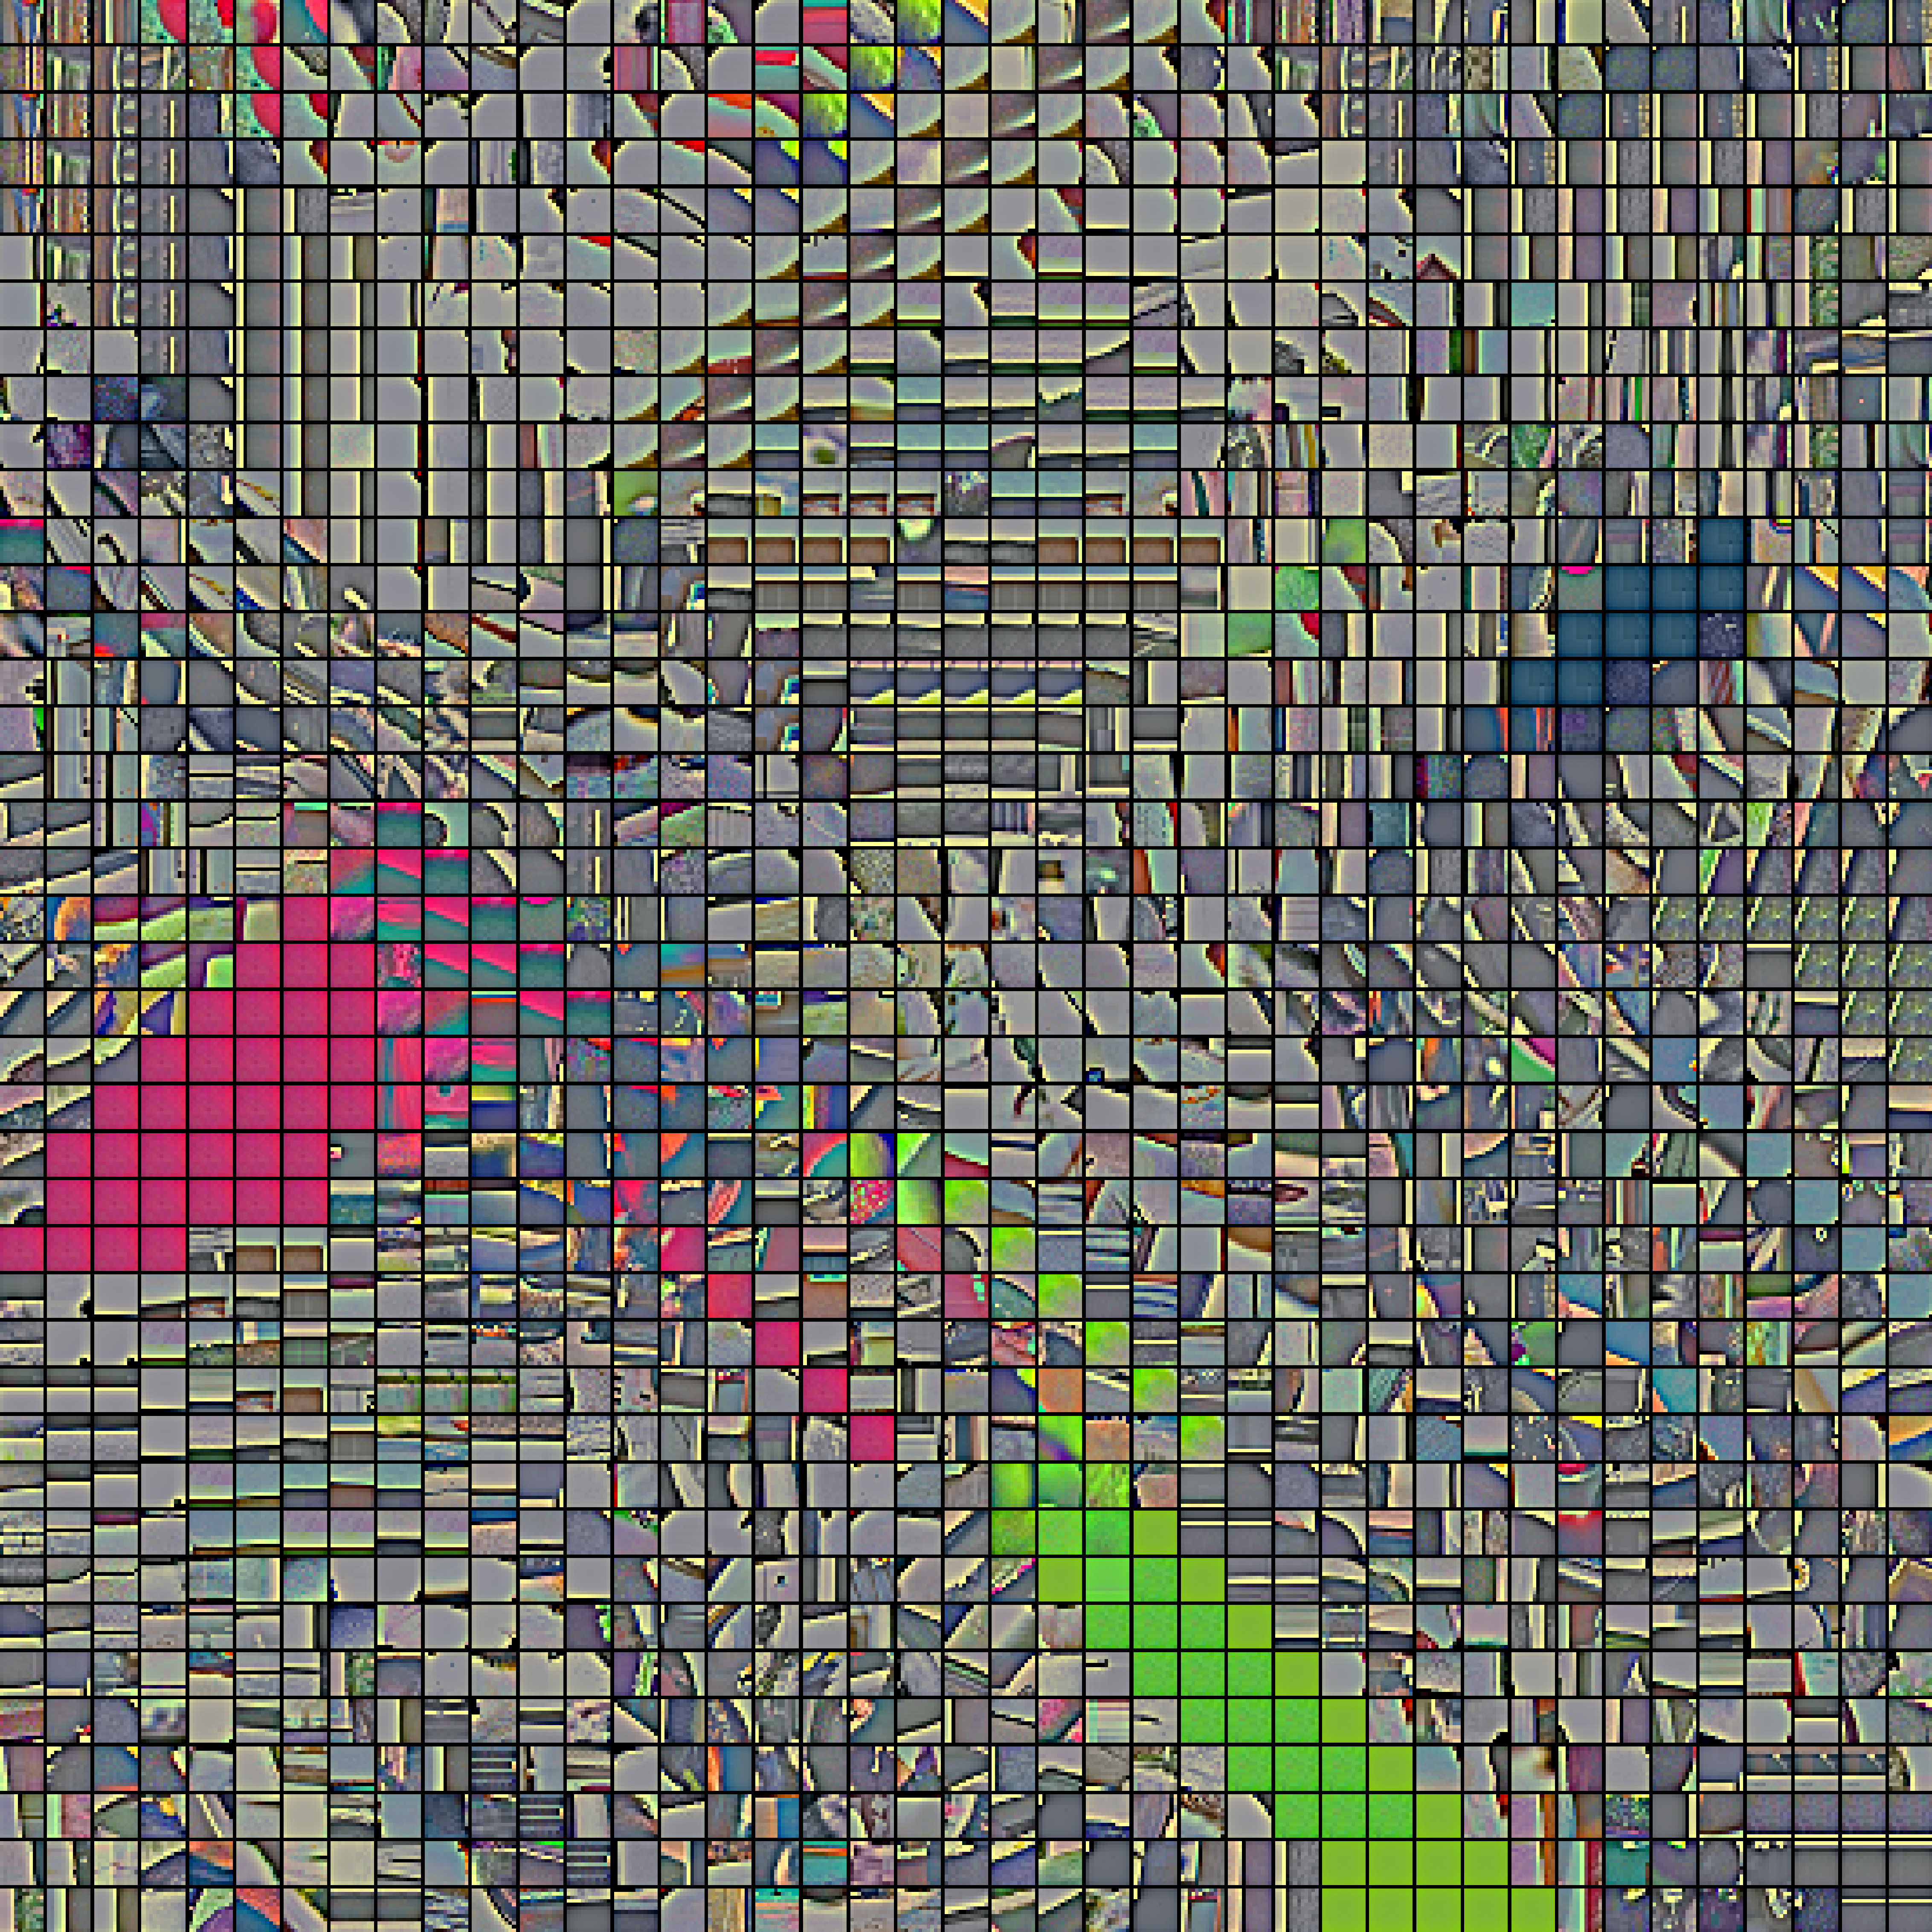
\includegraphics[width=0.32\linewidth]{figures/topographical_order_more_patches_imagenet128_patches_12}
  	  	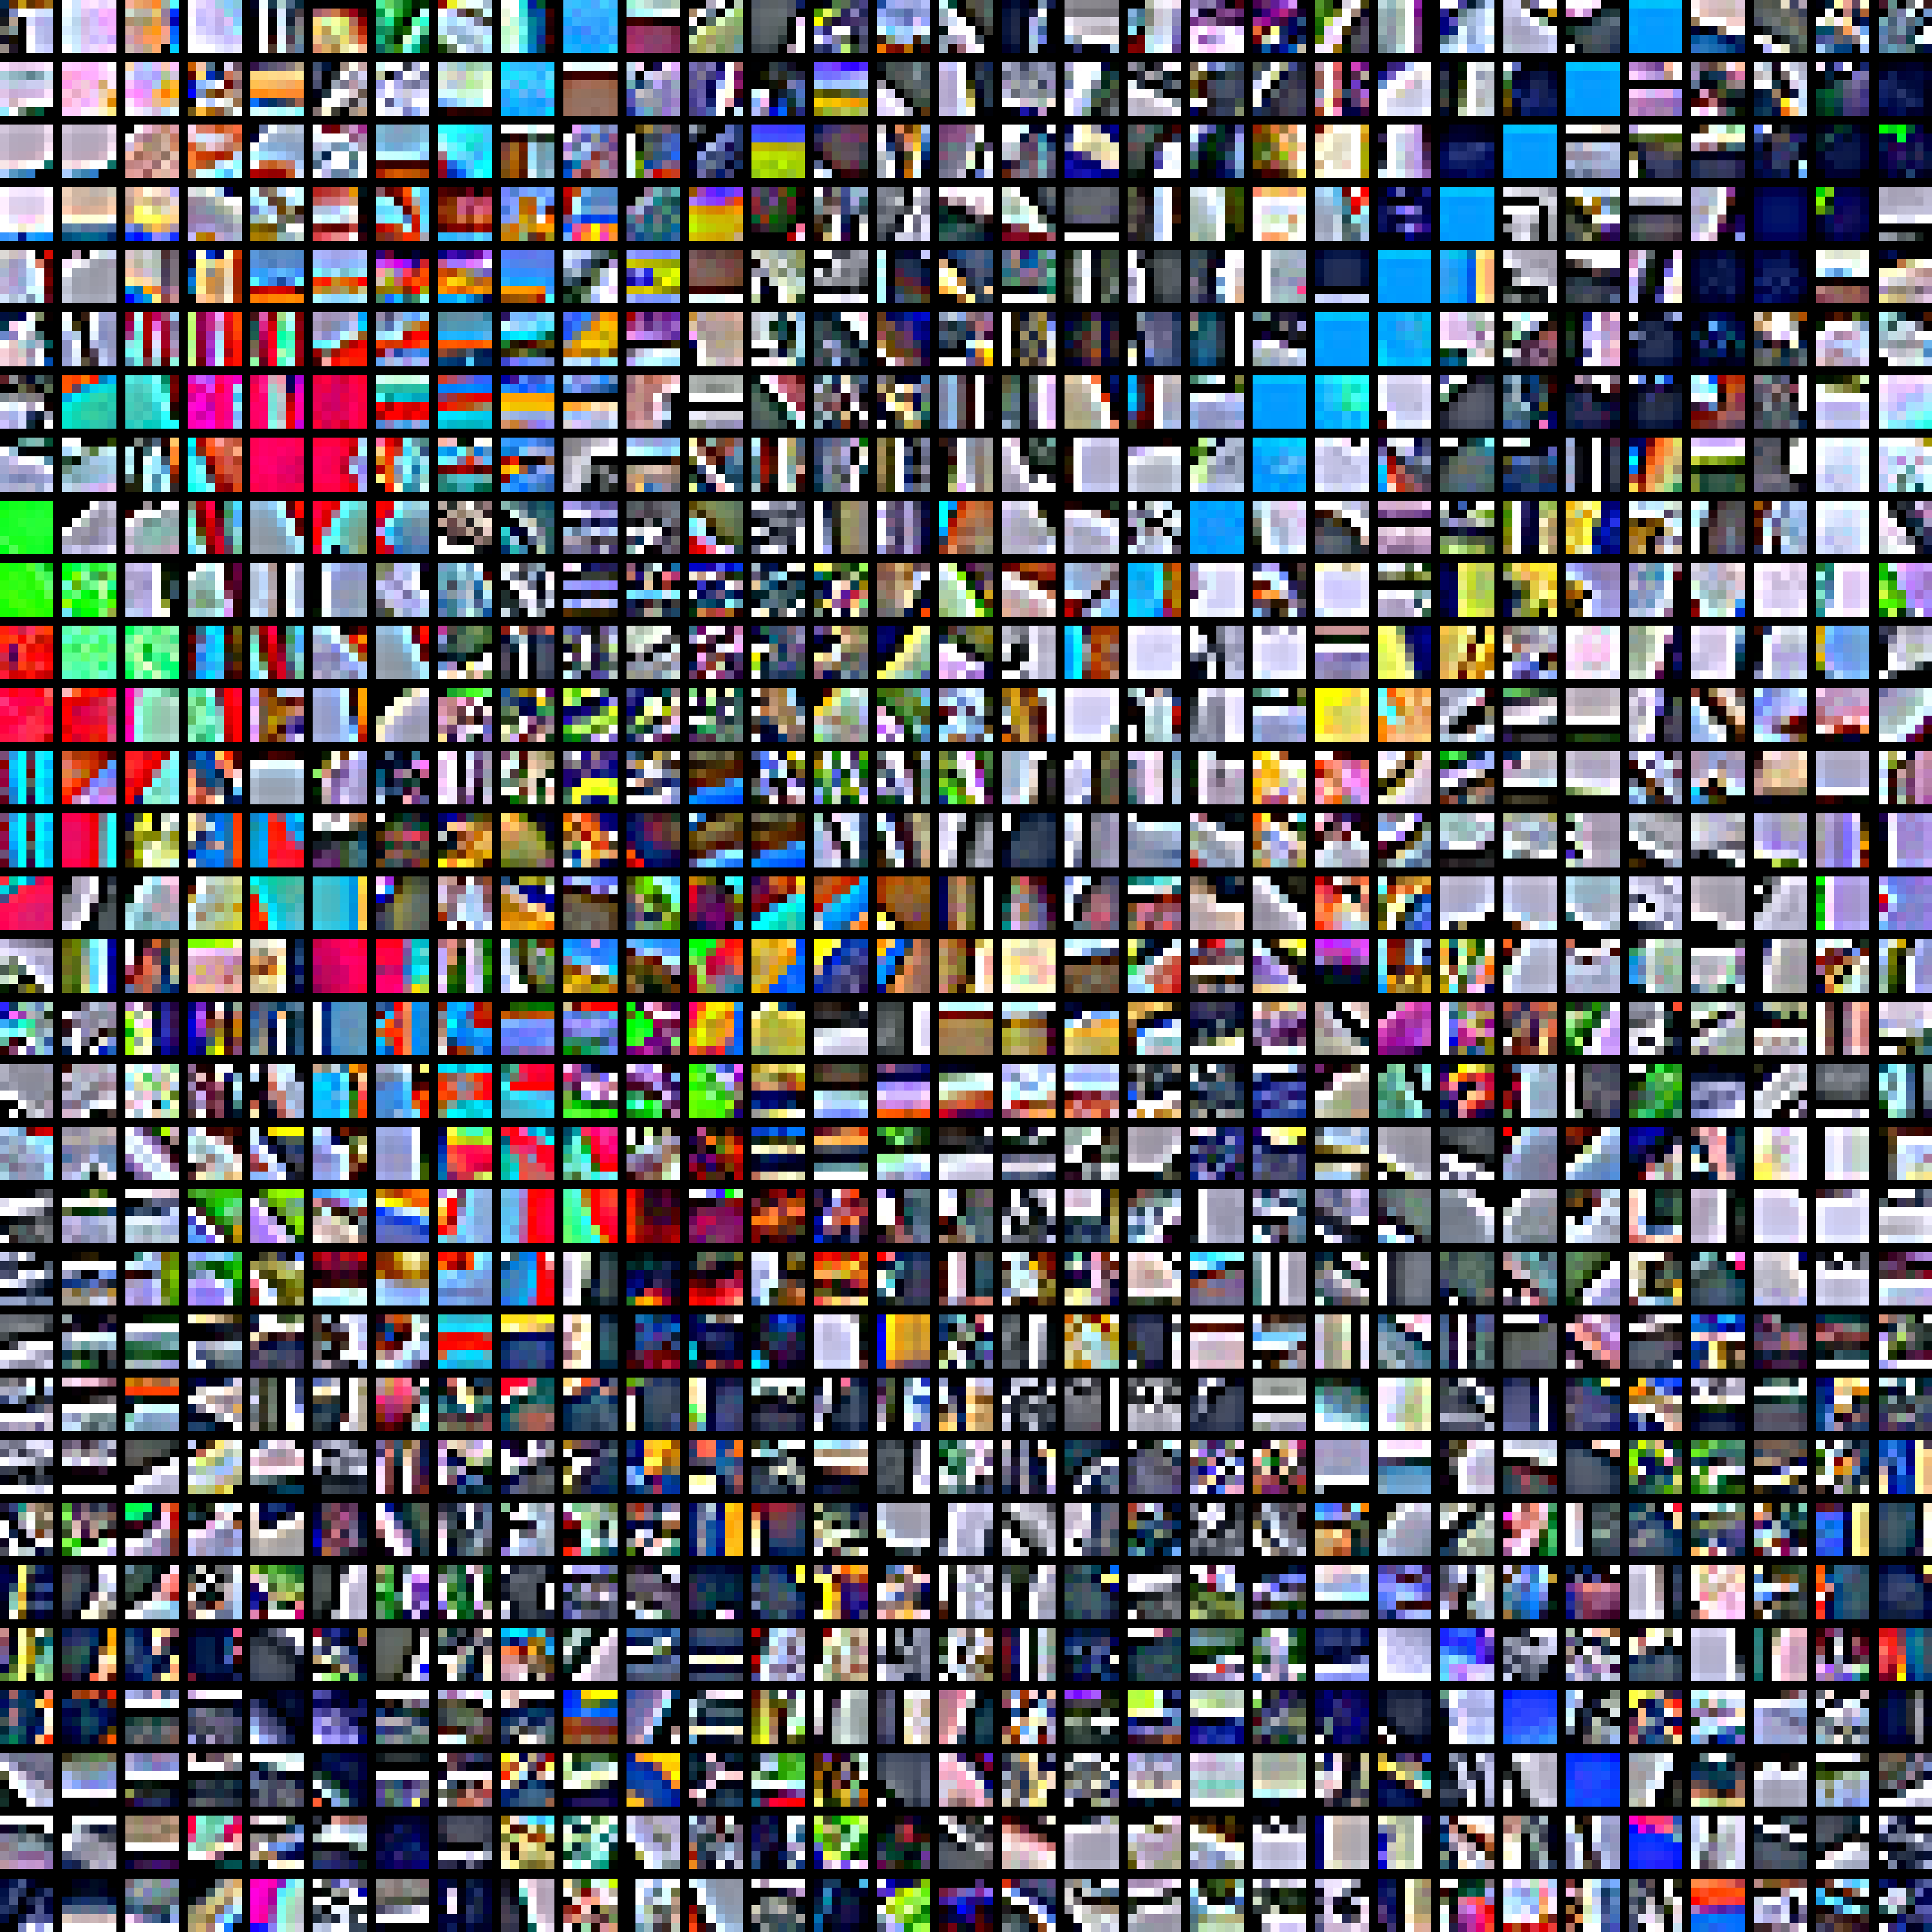
\includegraphics[width=0.32\linewidth]{figures/topographical_order_more_patches_imagnet64_patches_6_30Images}
  	  	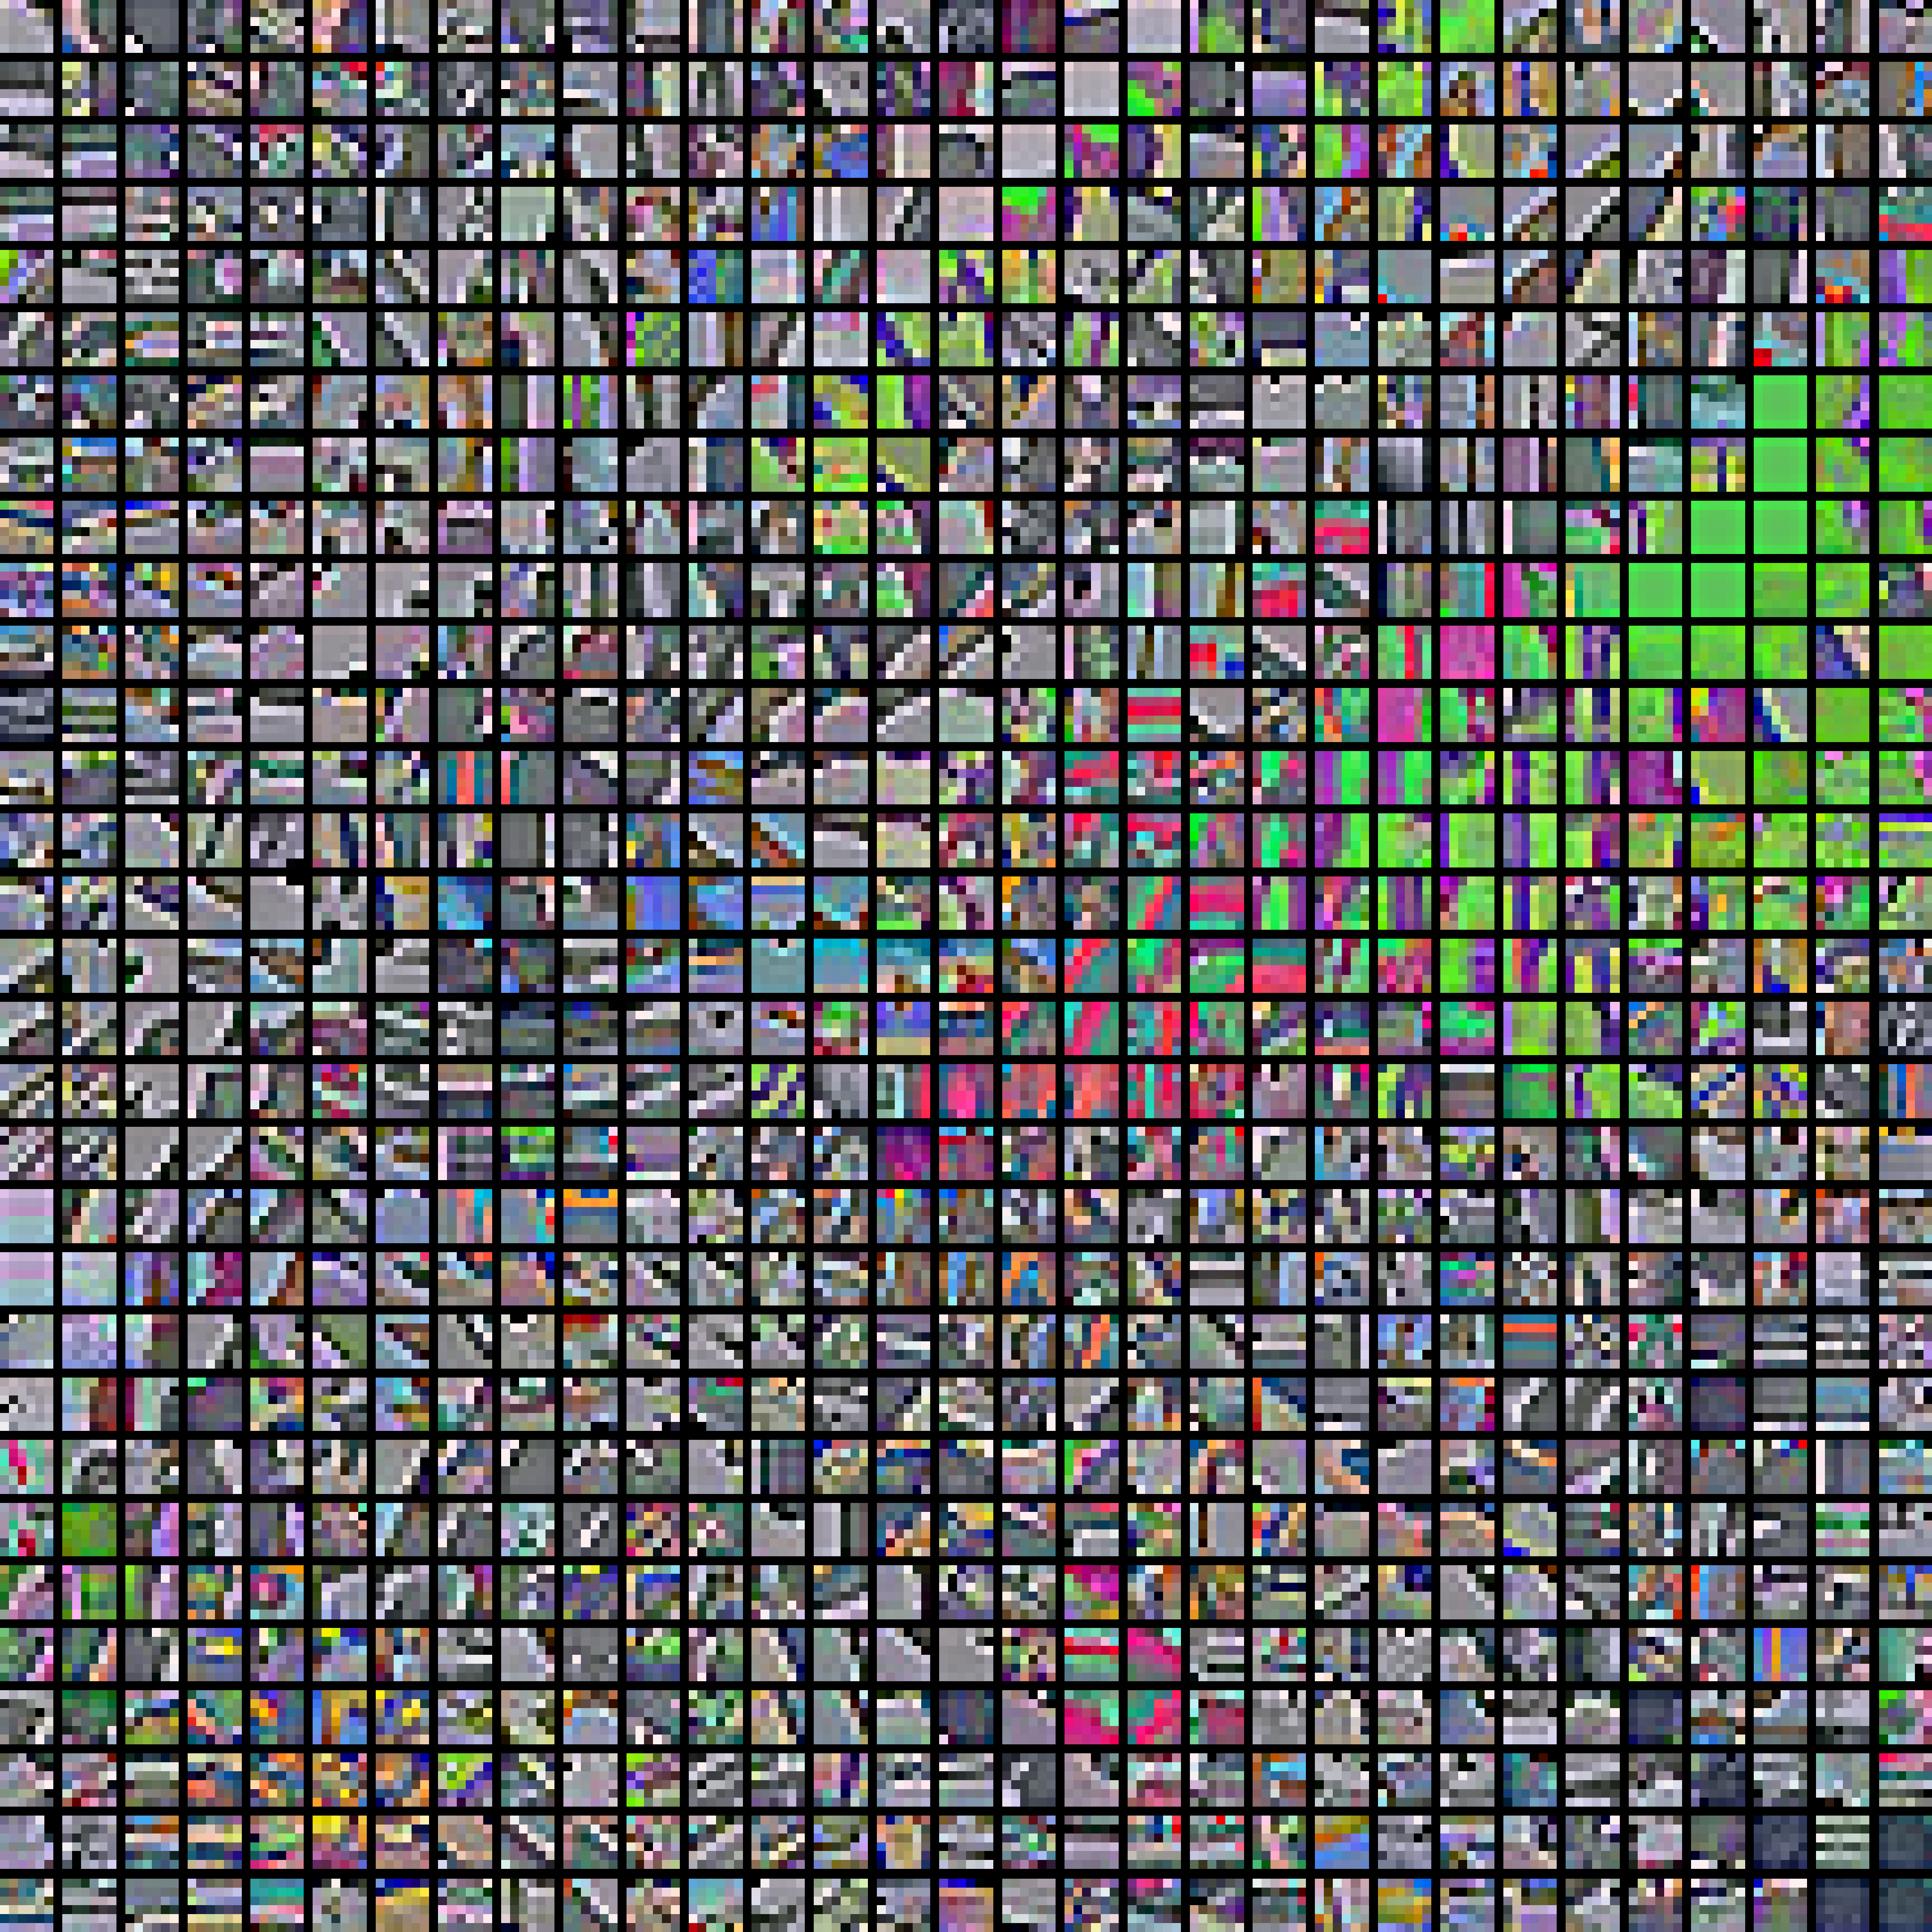
\includegraphics[width=0.32\linewidth]{figures/topographical_order_more_patches_cifar10_patches_6_30images}
\caption{An example of whitened dictionary  $\mathcal{D}$ from ImageNet-128 (Left), ImageNet-64 (Middle), CIFAR-10 (Right). The atoms have been reordered via a topographic algorithm and contrast adjusted.}
\label{dico}
\end{figure}

\subsection{$K$-Nearest Neighbors on patches\label{knn}}
The core idea of our algorithm is to compare the distances between each patches of an image and a fixed dictionary of patches $\mathcal{D}$, with size $|\mathcal{D}|$.
For a fixed dataset, this dictionary $\mathcal{D}$ is obtained by uniformly sampling patches from images over the whole training set. We augment $\mathcal{D}$ into $\cup_{d\in \mathcal{D}}\{d,-d\}$ because it allows the dictionary of patches to be contrast invariant and we observe it leads to better classification accuracies; we still refer to it as $\mathcal{D}$. An illustration is given by Fig.~\ref{dico}. Once the dictionary $\mathcal{D}$ is fixed, for each patch $p_{i,x}$ we consider the following set of  pairwise norms:
\begin{align}\mathcal{C}_{i, x} =\{\Vert p_{i, x} - d \Vert\,, d\in\mathcal{D} \}\,.\end{align}

 
For each whitened patch we encode the $K$-Nearest Neighbors of $p_{i,x}$ from the set $\mathcal{D}$, for some $ K \in \mathbb{N}$, which is a Vector Quantization (VQ) step with hard-assignment \Edouard{CITE}.
More formally, we consider $\tau_{i,x}$ the $K$-th smallest  element of $\mathcal{C}_{i,x}$, and we define the $K$-Nearest Neighbors binary encoding as follow, for $(d,i)\in\mathcal{D}\times\mathcal{I}$:


\begin{equation}
\label{encoding}
\phi(x)_{d,i}=
\begin{cases}
1,&\text{if } \Vert  p_{i,x} - d\Vert \leq \tau_{i,x}\\
0,&\text{otherwise}.
\end{cases}
\end{equation}


This representation thus encodes the patch neighborhood in a subset of randomly selected patches and can be seen as a crude description of the topological geometry of the image patches.
Moreover, it allows to view the distance between two images $x,y$ as a Hamming distance between the patches neighborhood encoding as:
\[\sum_{i,d}\Vert \phi(x)_{d,i}-\phi(y)_{d,i}\Vert^2=\sum_{i,d}\mathbf{1}_{\phi(x)_{d,i}=\phi(y)_{d,i}}\,.\]
It can also be seen as the output of a 1-hidden layer neural network, except that the non-linearity is not point-wise.

In order to reduce the computational burden of our method, we perform an intermediary average-pooling step.
Indeed, we subdivide $\mathcal{I}$ in squared overlapping regions $\mathcal{I}_j\subset\mathcal{I}$, leading to the representation $\Phi$ defined, for $d\in\mathcal{D}, j$ by:
\begin{align}\Phi(x)_{d,j}= \sum_{i\in \mathcal{I}_j}\phi(x)_{d,i}\,.\end{align}

The next section describes our classification pipeline, as we feed our representation $\Phi$ to a linear classifier on challenging datasets.
Note that due to the hard assignment  in VQ, it would not be possible to learn the parameters of our dictionary via a standard differentiable method, consequently this approach fails to be analyzed directly through the scope of \cite{chizat2018global} for instance.




\section{Experiments}
\label{experiments}
We train  shallow classifiers (e.g., Linear and 1-hidden layer CNNs) on top of our representation $\Phi$ on two major  image classification datasets,  CIFAR-10 and ImageNet, which consist respectively of $5\times10^5$ small and $1.2\times10^6$ large color images  divided respectively in 10 and $10^3$ classes.


\paragraph{Classifier parametrization} In each experiments, the spatial subdivisions $\mathcal{I}_j$ are implemented as an average pooling with kernel size $k_1$ and stride $s_1$.
We then apply a 2D batch-normalization \citep{ioffe2015batch} in order to standardize our features on the fly before feeding them to a linear classifier.
In order to reduce the memory fooprint of this linear classifier (following the same line of idea of a "bottleneck" \citep{he2016deep}), we factorize our linear classifier into two convolutional operators followed by a global average pooling with no-padding).  The first convolutional layer  consists of  convolutions with kernel size $k_2$ and stride 1 that reduces the number of channels from $\mathcal{D}$ to $c_2$. 
We then apply a  convolution with kernel size $k_3$ and stride 1 that outputs a number of channel equal to the number of image classes, followed by a global average pooling.
For the 1-hidden layer experiment, we  add a ReLU non linearity between the first and the second convolutional layer.

During each experiments,  our linear classifier is trained via mini-batch SGD with momentum of 0.9, no weight decay and the standard cross-entropy loss. We further employed a standard data augmentation, however, we reduced the image resolution for ImageNet, which we discuss below. We also arbitrily used $K=0.4 |\mathcal{D}|$, which implies that our representation is not sparse.



\subsection{CIFAR-10}

 \paragraph{Implementation details} Our linear operators are parametrized as follow: first, we used $k_1=5,s_1=3,k_3=6,Q=6$.
 Then, for the linear experiments and 1-hidden layer experiments, we used respectively $n_2=1, c_2=128$ and  $ n_2=3,c_2=1024$ because we observed it lead to better performances.
Our data augmentation consists in horizontal random flips and random crops of size $32^2$ after  reflect-padding with $4$ pixels.

We tested various size of $|\mathcal{D}|$. For $|\mathcal{D}|=2. 10^3$, the model is trained for 80 epoch with an initial learning rate of 0.003 decayed by 10 at epochs 50 and 75.
For  $|\mathcal{D}|=1.10^4$ or $|\mathcal{D}|=6. 10^4$, the model is trained during 175 epochs with an initial learning rate 0.001 decayed by 10 at epochs 100 and  150. 


\paragraph{Classification experiments} Our results are reported and compared in Tab.~\ref{cifar-acc}. 
First, note that contrary to experiments done by \cite{coates2011analysis} our methods has surprisingly good accuracy despite the hard-assignement in Vector Quantization.
Sparse coding, soft-thresholding and orthogonal matching pursuit based representations used by \cite{coates2011importance, recht2019imagenet} can be seen as soft-assignment VQ and yield comparable classification accuracy (resp. 81.5\% with $6.10^3$ patches and 85.6\% with $2.10^5$ patches).
However, these representations contain much more information than hard-assignment VQ as they allow to reconstruct a large part of the signal.
Our representation yields better accuracy with only topological information on the image patches, suggesting that this information is highly relevant for classification.
Moreover, we need a much smaller of patches than \cite{recht2019imagenet}, \cite{coates2011importance} or \cite{mairal2016end}, to obtain comparable accuracies, and using a 1-hidden layer classifier, our accuracy is competitive with deep kernel methods \citep{li2019enhanced,shankar2020neural} and deep supervised convolutional networks \citep{krizhevsky2012imagenet}.
This further indicates the relevance of patches topological information for classification task.



\begin{table}[h]
  \caption{Accuracies on CIFAR-10\label{cifar-acc}. Q is the patch size, $|D|$ the size of the patch dictionary and VQ indicates whether vector quantization with hard-assignment is applied. We observe that a linear classifier is sufficient to obtain high performance, demonstrated only with higher depth in other works. Compared to Recht et al our work shows that discarding information via hard-assignment VQ still allows to recover high performance. Amongst methods relying on random patches ours is the only approach operating online (and therefore allowing for scalable training). }
  \label{accuracy}
  \centering
  \begin{tabular}{|c|c|c|c|c|c|c|c|}
    \hline 
    Method&$|\mathcal{D}|$&VQ&Online &$Q$&Depth &Classifier& Acc. \\
    \hline 
    SimplePatch (Ours) &$2\cdot10^3$ & \checkmark&\checkmark &6&1&linear&82.5 \\
    \hdashline[0.5pt/1pt]
    SimplePatch (Ours) &$1\cdot10^4$ & \checkmark&\checkmark & 6&1&linear&85.6\\
    \hdashline[0.5pt/1pt]
    SimplePatch (Ours) &$6\cdot10^4$ & \checkmark&\checkmark &6&1&linear&86.6\\
    \hdashline[0.5pt/1pt]
    \cite{coates2011analysis}&$1\cdot10^3$& \checkmark& $\times$&6 & 1&linear & 68.6\\\hdashline[0.5pt/1pt]
   % \hline 
    \cite{recht2019imagenet}&$2\cdot10^5$ & $\times$&$\times$&6&1&linear &85.6\\
    \hdashline[0.5pt/1pt]
    CKN (\cite{mairal2016end})&$10^3, 10^4$& $\times$& $\times$&3 & 2& linear &85.8\\
    \hdashline[0.5pt/1pt]
    NK (\cite{shankar2020neural})&$\sim10^6$& $\times$& $\times$ &3&5&kernel &89.8\\
    \hdashline[0.5pt/1pt]
    NTK (\cite{li2019enhanced})&$2 \cdot 10^3$& $\times$&$\times$ &6&6&kernel &88.9\\\hdashline[0.5pt/1pt]
    Ours&$2\cdot10^3$ & \checkmark& \checkmark &6&2&1-NN&88.0\\
    \hline\hline
   % \hdashline[0.5pt/1pt]
    Scat. (\cite{Oyallon_2015_CVPR}) & - & $\times$& $\times$&8 &2 & kernel & 82.3\\ \hdashline[0.5pt/1pt]
    Alexnet (\cite{krizhevsky2012imagenet})&-& $\times$& \checkmark &-&5&end-to-end&89\\
    \hline
  \end{tabular}
\end{table}




\begin{figure} 
  
  \centering
   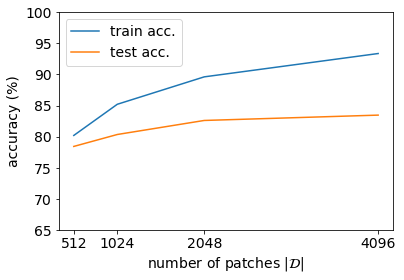
\includegraphics[width=0.35\linewidth]{figures/albation_study_npatches.png}
  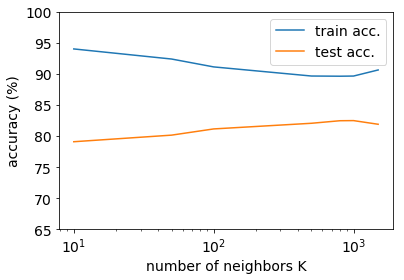
\includegraphics[width=0.35\linewidth]{figures/albation_study_K.png}
  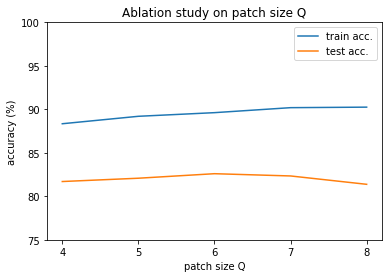
\includegraphics[width=0.35\linewidth]{figures/albation_study_Q.png}
  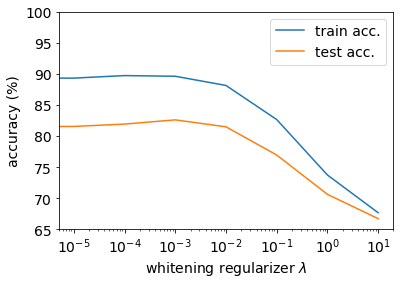
\includegraphics[width=0.35\linewidth]{figures/albation_study_lambda.png}\\
  \caption{CIFAR-10 ablation experiments on the number of patches  $|\mathcal{D}|$ (Top-left), the patch size $Q$ (Bottom-left), the number of neighbors $K$ (Top-right), the whitening regularizer $\lambda$ (Bottom-right).\label{fig:ablation_study}}
\end{figure}




\paragraph{Ablation experiments}
CIFAR-10 is a relatively small dataset that allows fast benchmarking, thus we conducted several ablation experiments in order to understand the relative improvement due to each hyper-parameters of our pipeline. We thus vary $|\mathcal{D}|$, $Q$, $K$ and $\lambda$ which are the hyper-parameters of $\Phi$. Results are shown in Fig. \ref{fig:ablation_study}.


% \Edouard{\sout{The starting experiment uses  $|\mathcal{D}|=2048$ patches, a patch size $Q=6$ a number of neighbors $K=0.4\times 2048 = 820$ and a whitening regularizer $\lambda=1e-3$.
% Note that our representation is absolutely not sparse.The number of patches $|\mathcal{D}|$ varies in $\lbrace 512, 1024, 2048, 4096 \rbrace$, the patch size $Q$ varies in $\lbrace 4, 5, 6, 7, 8 \rbrace$, the number of neighbors $K=
% $ varies in $\lbrace 10, 50, 100, 500, 800, 1000, 1500 \rbrace$ and  the whitening regularizer $\lambda$ varies in $\lbrace0, 10^{-5}, 10^{-4}, 10^{-3}, 10^{-2}, 10^{-1}, 1, 10\rbrace$.
% Results are shown in figure \ref{fig:ablation_study}.}}

Note that even a relatively small number of patches is competitive with much more complicated representation, such as \citet{Oyallon_2015_CVPR}.
We note that it is possible to slightly optimize the performances according to $K$ or $Q$, yet the fluctations remain minor compared to other factors, which indicate that the performances of our method are relatively stable w.r.t. this set of hyper-parameters. The Tykhonov regularization behaves similarly to a thresholding operator on the eigenvalues of $\Sigma^{1/2}$: the larger it is, the more it penalizes larger eigenvalues. Interestingly, we note that under a certain threshold, this hyper-parameter almost does not affect the classification performances. This goes in hand with both a fast eigen-value decay and a stability to noise, that we discuss further in Sec. \ref{structure}.
% \Edouard{\sout{Suprisingly, the whitening regularization $\lambda$ is not crucial as setting it to $0$ leads a $1\%$ drop in perfomance.
% Large values of $\lambda$ tend to cancel the whitening effect since the term $\lambda I$ dominates $\Sigma$ in the whitening operator $W = (\lambda I+\Sigma)^{-1/2}$.
% The accuracy drops severely for large values of $\lambda$, indicating that whitening is a key aspect of the representation.}}

\paragraph{Classifier factorization}
In order to test the inductive bias of our classifier, we  replace it with a simple fully connected layer, with $6$ times more parameters than ours: the train and test accuracies are $93.0\%$ and $81.6\%$ compared to $88.9\%$ and $82.5\%$. Thus, it significantly reduces overfitting, while reducing the number of computations. We note that the using convolutions is well motivated by the  structure of natural images (well-centered while their class is relatively invariant to translation).

\paragraph{Whitening and Gaussian random filters}As observed by some  works from Tab.~\ref{cifar-acc}, removing the whitening step leads to  a  performance drop  of about 17\%.
Similarly, using patches drawn from a standardized Gaussian distribution  instead of  the image patches leads to a drop of about 6\%. It indicates that both steps are crucial for obtaining our performances. 
Also, note that all these accuracies are significantly higher than the accuracy obtained with a linear classifier on the raw images ($\sim40\%$) yet they are below geometric representations like \cite{Oyallon_2015_CVPR}.

\paragraph{Impact of hard-assignment VQ}
Here, we replace the hard-assignment implemented with a binary non-linearity  $\mathbf{1}_{\Vert  p_{i,x} - d\Vert \leq \tau_{i,x}}$ (see Eq. \ref{encoding}) by a soft-assignment VQ with a sigmoid function $(1 + e^{\Vert  p_{i,x} - d\Vert - \tau_{i,x}})^{-1}$.
The accuracy increases by $0.4\%$, showing that the use soft-assignment in VQ that is crucial for perfomance in \cite{coates2011analysis,coates2011importance} does not affect much the performances of our representation.

\begin{figure}
\centering
  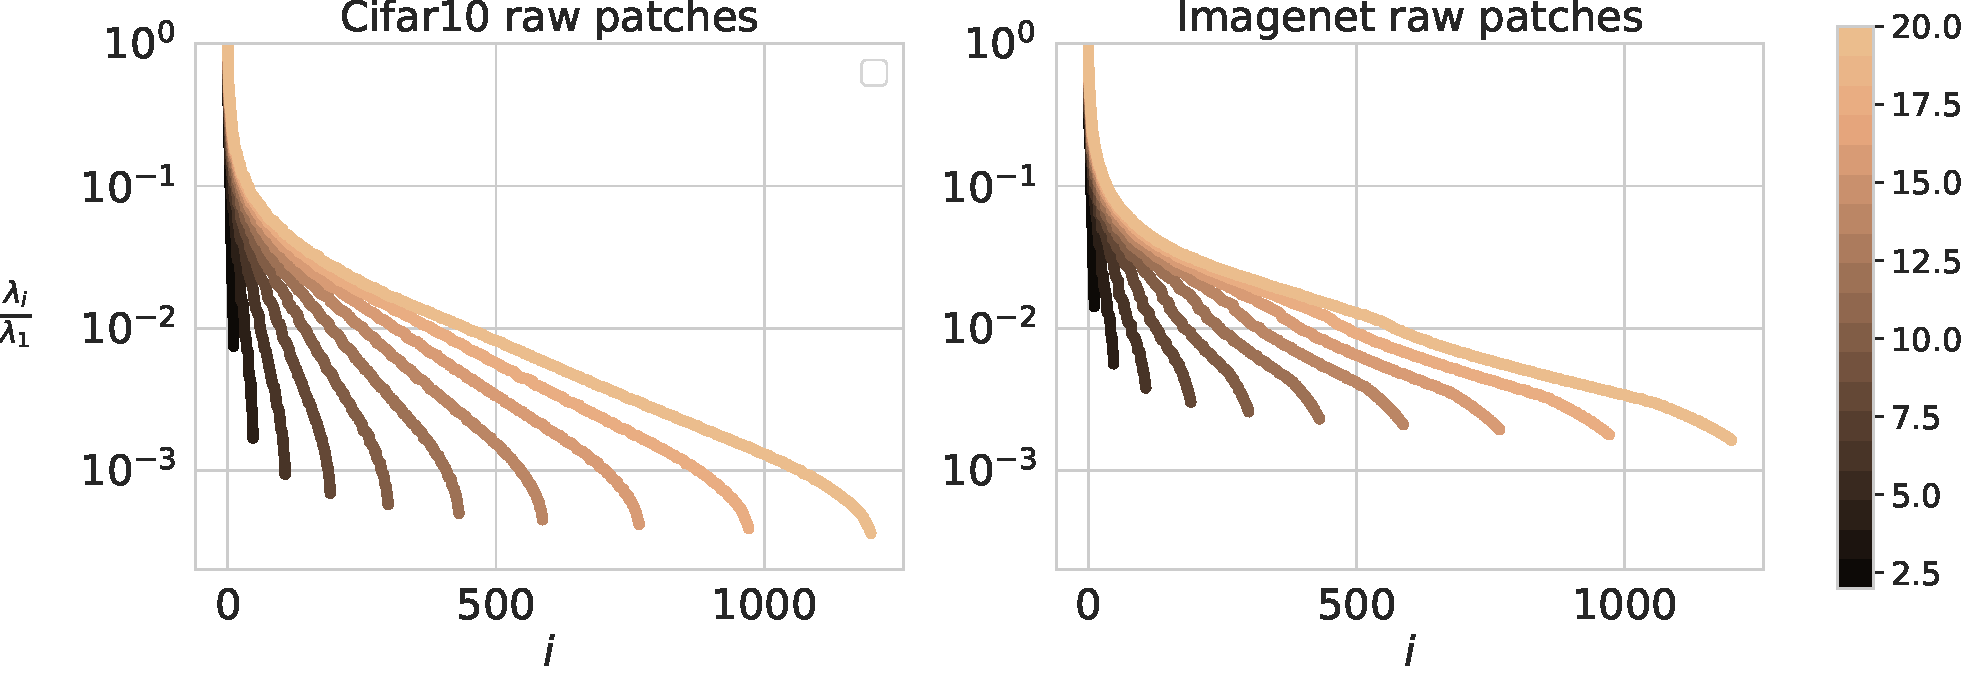
\includegraphics[width=.8\linewidth]{figures/spectrum_patches}
  \caption{Spectrum $\{\lambda_i\}_i$ of $\Sigma^{1/2}$ on CIFAR-10 (Left) and ImageNet-64 (Right).\label{spectrum} Colors encode the size of the patches $Q$: from dark brown for small patches to light brown to larger patches.}
\end{figure}
\subsection{ImageNet}

\paragraph{Implementation details}  Since ImageNet is a much larger dataset than CIFAR-10, we could  use no more than $|\mathcal{D}|=2048$ patches.
Here, $\lambda=10^{-2}, k_1=5,s_1=3, k_2=1, c_2=256, k_3=12, Q=6$. For the 1-hidden layer experiment, we used $k_2=3$.
In order to reduce the computational overhead of our method on ImageNet, we followed the same approach as \cite{DBLP:journals/corr/ChrabaszczLH17}. We reduce the resolution to $64^2$ as in \cite{DBLP:journals/corr/ChrabaszczLH17}, instead of the standard 224 length.  Note that \cite{DBLP:journals/corr/ChrabaszczLH17}  observed that this does not alterate much the top-performances of standard models ($5 \%$ to $10\%$ drop of accuracy on average), and we also believe it introduces a useful dimensionality reduction, as it removes high-frequency part of images that are  unstable
\citet{mallat1999wavelet}.
To measure the importance of the resolution on the performances, we also run a linear classification experiment on  ImageNet images with resolution $128^2$ using the same hyper-parameters except that we double the resolution of the initial operator (i.e., $Q=12, k_1=10,s_1=6$).

Our models are trained during 60 epochs with an initial learning rate of 0.003 decayed by a factor 10 at epochs 40 and 50.
During training, similarly to \cite{DBLP:journals/corr/ChrabaszczLH17} we use random flip and we select random crops of size of size $64^2$ , after a reflect-padding of size 8. At testing, we simply resize the image to $64^2$.
Note thas this procedure differs slighly from the usual data-augmentation, which consists in resizing images while maintaining ratios, before a random cropping.

%\paragraph{Imagenet64}

%We use a patch size $Q=6, P=64, R=8$.
%For the linear experiments, the linear layer hyperparameters are  $n_1=5,s=3, n_2=1, c=256, n_3=12$.






\paragraph{Classification experiments}
Tab.~\ref{imagenet-xp} reports the accuracy of our method, as well as the accuracy of comparable methods. Using small images still allows our method to outperform by a large margin ( about $\sim 10\%$ Top-5) the  Scattering Transform \citep{mallat2012group}, which was the previous state-of-the-art-method in the context of no-representation learning. Note that it also outperforms randomly initialized neural networks \citep{arandjelovic2017look}.

Using multiple patch encoding steps (SIFT, Fisher kernel, power normalization, compression) , \cite{sanchez2013image} obtain $72.0\%$ top-5 accuracy using a patch representation of dimension $6.10^4$ and $64.1\%$ top-5 accuracy using a patch representation of dimension $4.10^3$.
Our method tested on lower resolution images using a representation of dimension $2.10^3$ ($=|\mathcal{D}|$) explains a large part of the perfomance of the $4.10^3$ dimensional Fisher Vectors, but proper large scale experiements would be needed to seed if it holds for $6.10^4$ dimensional Fisher Vectors.
Still, a major difference between our representation and both Scattering Transform and Fisher Vector is the hard-assignment VQ that discards signal information while the image can be fairly reconstructed using Scattering coefficients \citep{oyallon2017scaling} or SIFT descriptors \citep{weinzaepfel2011reconstructing}.


We now compare our performances with supervised models trained end-to-end.
BagNets \citep{brendel2019approximating} have shown that  competitive classification accuracies can be obtained with patch-encoding that consists of 50 layers.
The perfomance obtained by our shallow experiment with a 1-hidden layer classifier reduces significantly the gap of performance between our method and a BagNet with similar patch-size.
This suggests once again that hard-assignment VQ does not degrade much of the classification information.
We also note that our approach with a linear classifier outperforms other supervised shallow baseline that consists of 1 or 2 layers \citep{belilovsky2018greedy}, which indicates that a patch based representation is a non-trivial baseline.

We also observe that using $128^2$ images improves our classification performances.
Note that the patches used are in a space of dimension $12^2 \times 3 = 432 \gg 1$:  our performance is surprising given that  nearest neighbors are known to be meaningless in high-dimension \citep{beyer1999nearest}.
This shows a form of low-dimensionality in the natural image patches, that we study in the next Section.




\begin{figure}\center
	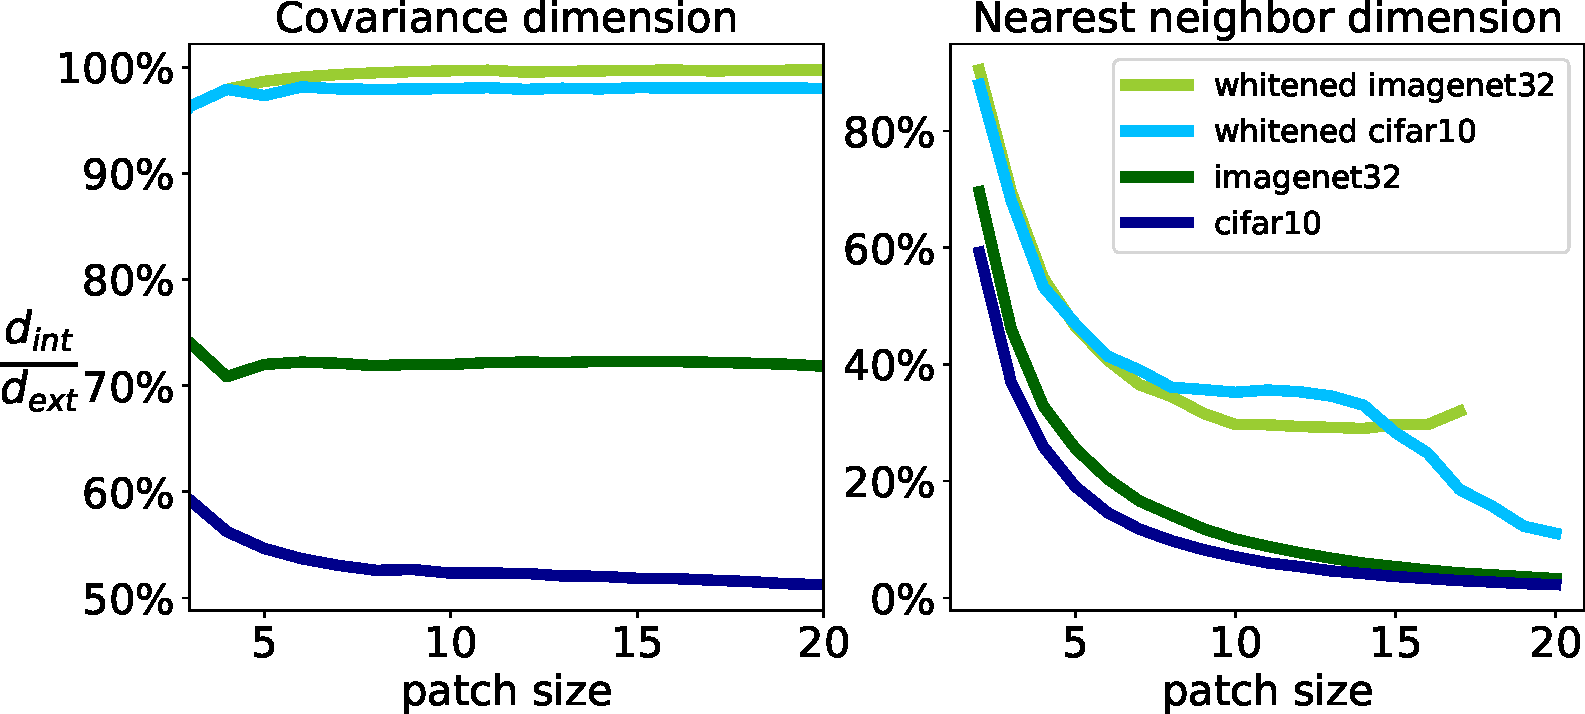
\includegraphics[width=.9\linewidth]{figures/intrinsic_dims}
	\caption{(Left) Ratio between covariance dimension and extrinsic dimension of the patches as a functions of their size. (Right) Ratio between nearest neighbor dimension and extrinsic dimension of the patches as a functions of their size.}
	\label{fig:intrinsic_dim}
\end{figure}

%\paragraph{Random filters and whitening} On Imagenet64, removing the whitening step leads to an accuracy of $18\%$ top-1, i.e. a drop of about 16\%. Like for Cifar-10, this step is crucial for performance.

\begin{table}[h]
  \caption{Accuracies on ImageNet, e-to-e, Res., Classif. and sup. stand respectively for end-to-end, Resolution, Classifier and supervised.\label{imagenet-xp}}
  \label{accuracy}
  \centering
  \begin{tabular}{|c|c|c|c|c|c|c|c|c|c|}
    \hline 
    Reference&Name& $|\mathcal{D}|$&VQ & $Q$ & Depth & Res. & Classif. & Top1&Top5 \\
    \hline 
    \hline
    Ours&Patch&$2.10^3$& \checkmark & 6 & 1 & 64 & linear & 33.4 &  54.7 \\
    \hdashline[0.5pt/1pt]
    Ours  &Patch&$2.10^3$& \checkmark & 12 & 1 & 128 & linear & 35.4  &  56.9 \\
    \hdashline[0.5pt/1pt]
    \cite{zarka2019deep}&Scatt. & -& $\times$ & 32 & 2 & 224 & linear & 26.1  & 44.1 \\
    \hdashline[0.5pt/1pt]
    \cite{arandjelovic2017look}&Random & - &$\times$& - &9 & 224 & linear & 18.9  & -\\
    \hline
    \cite{sanchez2013image} & FV& - &$\times$& 24 & 4 & full& linear & - & \Edouard{72.0}\\
    \hline
     Ours &Patch& $2.10^3$ & \checkmark & 6 & 2 & 64 & 1-NN & 39.4 &  62.1 \\
     \hdashline[0.5pt/1pt]
   \cite{belilovsky2018greedy}&Shallow&-&$\times$&-&1&224&e-to-e&-&26\\
    \hdashline[0.5pt/1pt]
   \cite{belilovsky2018greedy}&Shallow&-&$\times$&-&2&224&sup.&-&44\\
   \hline
   \cite{brendel2019approximating} & BagNet & - &$\times$& 9 & 50 & 224 & e-to-e & - & 70.0
    \\
    \hdashline[0.5pt/1pt]
    \cite{krizhevsky2012imagenet}& AlexNet&-&$\times$&-&10&224&e-to-e&59.3&81.8\\
   \hline
  \end{tabular}
\end{table}









\subsection{Dictionary structure}
\label{structure}
\paragraph{Spectrum of $\mathcal{D}$}
Fig. \ref{spectrum} shows the spectrum of $\Sigma^{1/2}$ for  sizes $Q$, normalized by $\Vert \Sigma^{1/2}\Vert$ on CIFAR-10 and ImageNet-32.  First, note that the spectrum tends to decay at an exponential rate (linear rate in semi-logarithmic scale). This rate decreases as the size of the patch increases (from dark brown to light brown) suggesting an increased linear dimensionality for larger patches. The second observation is that patches from ImageNet-32 dataset tend to be better conditioned than those from CIFAR-10 with a conditioning ratio of $10^2$ for ImageNet vs $10^3$ for CIFAR-10. This is probably due to the use of more diverse images than on CIFAR-10. From this spectrum, it is straightforward to compute the linear dimensionaity of the patches. Fig.
~\ref{fig:intrinsic_dim} shows the number of axis needed to explain $95\%$ of the variance as a function of $Q^2$, with and without whitening. Before whitening, this linear dimension is much smaller than the ambient dimension: whitening the patches increase the linear dimensionality of the patches, which still decrease at a linear growth as a function of $Q^2$.

\paragraph{Intrinsic dimension of $\mathcal{D}$}
We propose to refine our measure of linear dimensionality to a non-linear measure of the intrisc dimension. Indeed, under the assumption of low-dimensional manifold, the linear dimensionality is simply an upper bound of the true dimensionality of the data. To do so, we employ the method introduced in \citep{Levina:2004}. We first estimate a local intrinsic dimension near a particular patch $p$ using the following analytic expression:
\begin{align}
	d_{int}(p) = \left( \frac{1}{K-1} \sum_{k=1}^{K-1}\log \frac{\tau_K(p)}{\tau_k(p)} \right)^{-1} \, ,
\end{align}
where $\tau_k(p)$ is the euclidean distance between the patch $p$ and it's $k$-th nearest neighbor from the training set. 
An overall estimate of the $d_{int}$ is then obtained by averaging the local estimate $d_{int}(p)$ over all patches. Such estimate depends on the maximum number of neighbors $K$. However, it converges to the same value when both $K$ and the size of the dataset  increases, provided that $K$ remains small compared to it. Fig. \ref{fig:intrinsic_dim} (right) shows the intrinsic dimension estimated using $K=2000$. It is clear that the estimated dimension $d_{int}$ is much smaller than the ambient dimension $Q
^2$ in all cases. Moreover, it grows even more slowly than the linear dimension when the patch size $Q$ increases. Finally, even after whitening, $d_{int}$ is only about $30\%$ of the total dimension, which is a strong evidence that the natural image patches are low dimensional.    
\section{Conclusion}

In this work, we have introduced a new visual reprensentation for image classification based on patches nearest neighbors encoding for Euclidian distance.
This representation, that has not been optimized nor learned achieves a competitive accuracy on CIFAR-10 and can be easilly scaled to large datasets such as ImageNet, yielding a non trivial performance.%\Edouard{ We note that this solution addresses the forgetting issue}. % I would add this


Due to limited computational ressources, we restricted ourselves on ImageNet to small image resolution (64 - 128) and to a relatively small number of patches (2048 patches out of the billions of patches of  Imagenet).
Conducting proper large scale experiments is thus one of the next research direction.
Ablation studies indicate that the success of the method lies on the use of the Mahanalobis distance, i.e. the whitening of the patches rather than the canonical Euclidean distance.
As this distance might not be optimal for classification, another direction of research is to learn a Mahanalobis distance by gradient descent for classification.




\bibliographystyle{abbrvnat}
\bibliography{biblio}{}

\newpage

\appendix

\section{Mahanalobis distance and whitening}

The Mahalanobis distance \citep{chandra1936generalised, mclachlan1999mahalanobis} between two samples $x$ and $x'$ drawn from a random vector $X$ with covariance $\Sigma$ is defined as  
\begin{align*} D_M (x, x' ) =  \sqrt{ (x - x')^T \Sigma^{-1} (x - x')} \end{align*}
If the random vector $X$ has identity covariance, it is simply the usual euclidian distance : 
\begin{align*} D_M (x, x' ) =  \| x - x' \| \ .\end{align*}

Using the diagonalization of the coraviance matrix,  $\Sigma = P\Lambda P^T$, the affine whitening operators of the random vector $\mathbf{X}$ are the operators 
\begin{equation}
\label{whitening}
     w : \mathbf{X} \mapsto O \Lambda^{-1/2} P^T (\mathbf{X} - \mu), \quad \forall O \in  O_n (\mathbb{R}) \ .
\end{equation}
For example, the PCA whitening operator is 
\begin{equation*}
     w_{\rm PCA} : \mathbf{X} \mapsto \Lambda^{-1/2} P^T (\mathbf{X} - \mu)
\end{equation*}
and the ZCA whitening operator is 
\begin{equation*}
     w_{\rm ZCA} : \mathbf{X} \mapsto P \Lambda^{-1/2} P^T (\mathbf{X} - \mu) \ .
\end{equation*}
For all whitening operator $w$ we have :
\begin{align*}
\|w(x) - w(x')\| = D_M(x, x') \ .
\end{align*}
Indeed 
\begin{align*}
  \|w(x) - w(x')\|
    &= \| O \Lambda^{-1/2} P^T ( x - x') \|\\
    &= \sqrt{(x - x')^T P \Lambda^{-1/2} O^T O \Lambda^{-1/2} P^T (x - x') }\\
    &=  \sqrt{ (x - x')^T P \Lambda^{-1} P^T (x - x')} \\
    &= D_M(x, x') \ .
\end{align*}

\section{Implementation of the K nearest neighbors as a 1 layer convolutional network}

In this section, we explicitely write the whitened patches with the whitening operator $W$.
Recall that  we consider the following set of euclidean pairwise distances:
\begin{align*}\mathcal{C}_{i, x} =\{\Vert W p_{i, x} - W d \Vert\, d\in\mathcal{D} \}\,.\end{align*}

For each image patch we encode the $K$ nearest neighbors of $W p_{i,x}$ in the set $Wd, d \in \mathcal{D}$, for some $ K \in 1 \ldots|\mathcal{D}| $.

Using the square distance instead of the distance doesn't change the $K$ nearest neighbors.
We have 
\begin{align*} \Vert Wp_{i,x} - Wd \Vert^2 = \Vert Wp_{i,x} \Vert^2 - 2 \langle p_{i,x}, W^T W d \rangle + \Vert Wd\|^2 \end{align*}
The term $\|Wp_{i,x}\|^2$ doesn't affect the $K$ nearest neighbors, so the $K$ nearest neighbors are the $K$ smallest values in
\begin{align*}
        \|Wd \|^2 - 2\langle p_{i,x}, W^T W d \rangle
\end{align*}
or equivalently the  $K$ largest values in

\[
        \langle p_{i,x}, W^T W d \rangle - {\|Wd \|^2 \over 2} 
\]
This can be implemented in a convolution of the image using $W^T W d$ as filters and ${\|Wd \|^2 \over 2}$ as bias term, followed by a vectorwise non-linearity that binary encodes the $K$ largest values in the channel dimension.

To compute the $K$ nearest neighbors in $\mathcal{D}$ we have to compute the quantity
\begin{align*} \langle p_{i,x}, W^T W d \rangle - {\|Wd \|^2 \over 2} \end{align*}
We can then easily compute 
\begin{align*} - \langle p_{i,x}, W^T W d \rangle - {\|Wd \|^2 \over 2} \end{align*} which is the quantity needed to compute the $K$ nearest neighbors in the set of negative patches $\overline{\mathcal{D}}$.
This is a cheap way of doubling the number of patches.


\end{document}
